%%%%%%%%%%%%%%%%%%%%%%%%%%%%%%%%%%%%%%%%%%%%%%%%%%%%%%%%%%%%%%%%%%%%%%

% From jcapexample.tex
\RequirePackage[displaymath]{lineno}
\documentclass[a4paper,11pt]{article}
\pdfoutput=1 

% JCAP style
\usepackage{jcappub}
\usepackage[T1]{fontenc} % if needed
%\usepackage{lineno}



% Stuff not in jcappub
\usepackage{aas_macros}
%\usepackage{xcolor}
\usepackage{tablefootnote}
\usepackage[displaymath]{lineno}
\usepackage{subfigure}
\usepackage{multirow}
\usepackage{amsmath}


%% Language and font encodings
%\usepackage[english]{babel}
%\usepackage[utf8x]{inputenc}
%\usepackage[T1]{fontenc}

\usepackage{enumitem}
\newcommand{\subscript}[2]{$#1 _ #2$}
%% Sets page size and margins
%\usepackage[a4paper,top=3cm,bottom=2cm,left=3cm,right=3cm,marginparwidth=1.75cm]{geometry}

%% Useful packages
%\usepackage{amsmath}
\usepackage{graphicx}
\usepackage[colorinlistoftodos]{todonotes}
%\usepackage[colorlinks=true, allcolors=blue]{hyperref}

%\usepackage{footmisc}
%\renewcommand\footnotelayout{\fontsize{10}{12}\selectfont}

\notoc


% Latex macros
%\input{fermiStyle.tex}




%%%%%%%%%%%%%%%%%%%%%%%%%%%%%%%%%%%%%%%%%%%%%%%%%%%%%%%%%%%%%%%%%%%%%%%%

\def\ie{{\it i.e.}}
\def\lsim{\:\raisebox{-0.5ex}{$\stackrel{\textstyle<}{\sim}$}\:}
\def\gsim{\:\raisebox{-0.5ex}{$\stackrel{\textstyle>}{\sim}$}\:}
\def\half{\textstyle{1\over2}}
\def\fouth{\textstyle{1\over4}}
\def\eighth{\textstyle{1\over8}}
\def\third{{\textstyle{1 \over 3}}}
\topmargin 1cm

\newcommand{\GEV}{\ensuremath{\,\textnormal{GeV}}}
\newcommand{\TEV}{\ensuremath{\,\textnormal{TeV}}}
\newcommand{\MEV}{\ensuremath{\,\textnormal{MeV}}}
\newcommand{\KEV}{\ensuremath{\,\textnormal{KeV}}}
\newcommand{\SEC}{\ensuremath{\,\textnormal{s}}}
\newcommand{\dropbox}{/Users/nicoviaux/Dropbox/} %Cambiar esta linea para editar
\newcommand{\folder}{Gravitino_Bounds/Paper/}
%\newcommand{\folder}{/media}

\newcommand*{\blue}{\textcolor{blue}}
\newcommand*{\red}{\textcolor{red}}

\interfootnotelinepenalty=10000


\begin{document}

\title{Gravitino dark matter with trilinear couplings to explain the anomalous positron fraction}

% Author list
\author[a,b]{Johannes~Buchner,}
\author[d]{Edson~Carquin,}
\author[c]{Marco~A.~D\'\i az,}
\author[a]{Germ\'an~A.~G\'omez-Vargas,\footnote{Now Corporate Data Scientist at \href{https://www.derco.cl/}{Derco},}}
\author[a]{Boris~Panes,}
\author[d]{Nicol\'as Viaux}

\affiliation[a]{Instituto de Astrof\'isica, Pontificia Universidad Cat\'olica de Chile, Avenida Vicu\~na Mackenna 4860, Santiago, Chile}
\affiliation[b]{Millenium Institute of Astrophysics, Vicu\~na MacKenna 4860, 7820436 Macul, Santiago, Chile}
\affiliation[c]{Instituto de F\'isica, Pontificia Universidad Cat\'olica de Chile, Avenida Vicu\~na Mackenna 4860, Santiago, Chile}
\affiliation[d]{Departamento de F\'isica y Centro Cient\'ifico- Tecnol\'ogico de Valpara\'iso (CCTVal), Universidad T\'ecnica Federico Santa Mar\'ia, Av. Espa\~na 1680, Valpara\'iso, Chile}

\emailAdd{johannes.buchner.acad@gmx.com} % orcid: 0000-0003-0426-6634
\emailAdd{edson.carquin@usm.cl}
\emailAdd{mad@susy.fis.puc.cl}
\emailAdd{ggomezv@uc.cl}
\emailAdd{bpanes@astro.puc.cl}
\emailAdd{nicolas.viaux@usm.cl}


%\pacs{95.35.+d,95.30.Cq,98.35.Gi}

\abstract{ The flux of charged leptons measured by the space-based detectors PAMELA, AMS-02, CALET, DAMPE and Fermi-LAT presents anomalous behavior as energy increase. In particular AMS-02 observations provide compelling evidence for a new source of positrons and electrons. Its origin is still unknown, but standard and successful scenarios include the contribution of dark matter and unresolved astrophysical sources, such as nearby pulsars. On the one hand, it has been shown that explanations based mostly on dark matter emission tend to overproduce gamma-rays, entering in conflict with measurements of the extra-galactic gamma-ray background (EGB). On the other hand, explanations using pulsars have shown good performance to solve the data, but these ideas are still under scrutiny. In general, a mixture of sources would signal a good approach for future research. However, before going deeply into that research direction, in this work we would like to present a dark matter scenario, which contains a gravitino as dark matter candidate with trilinear couplings to standard model particles, that is able to solve both the lepton data as well as the bounds from the EGB. Besides, it also offers some connections to other observables such as neutrino physics. These results may serve as a probe of concept for the dark matter only explanation of the positron anomaly, but more conservatively speaking it could motivates the use of this model for future mixed searches.} 

%\mathbf{on cosmic rays, }

\keywords{dark matter experiments, cosmic ray experiments, gamma ray experiments, dark matter theory}

\maketitle
%\flushbottom


\newpage
%%%%%%%%%%%%%%%%%%%%%%%%%%%%%%%%%%%%%%%%%%%%%%%%%%%%%%%%%%%%%%%%%%%%
\section{Introduction}
%%%%%%%%%%%%%%%%%%%%%%%%%%%%%%%%%%%%%%%%%%%%%%%%%%%%%%%%%%%%%%%%%%

The continuous and systematic analysis of the data collected by cosmic-ray detectors is one of the most direct ways to check and test the predictions of particle physics models that contain a candidate for dark matter which is meta-stable. The slow but acceptable decay rate of dark matter particles indeed can produce relevant fluxes of leptons, photons and heavy elements that can contribute to the number and features of detected events in current and future experiments, see \cite{Grefe:2011dp} for an extensive review focused on the gravitino dark matter scenario. 

Furthermore, this discussion becomes specially relevant since contemporary experiments show the presence of persistent and striking anomalies concerning the detection of cosmic-rays. For instance, the energy spectrum of electrons and positrons measured by experiments such as AMS-02, CALET, DAMPE and Fermi-LAT \blue{references for each dataset} show noticeable discrepancies when compared to standard predictions. \blue{Here, we may explain the main features of these standard models or we could have a short section for that}. Therefore, these experimental signals strongly suggest that extra sources of (primary) positrons are required in order to make sense of the data. 

From a revision of the latest literature concerning this subject we can conclude that the source of the charged lepton excess in general could be given by a mixture of dark matter and currently unresolved astrophysical sources, such as pulsars. \blue{Here, we may add some description of previous literature, just relevant references or we could discuss it in a short section}. Although we agree that future efforts should consider this mixture as working hypothesis, here we would like to re-consider the dark matter only solution. The discussion concerning the potential presence of unresolved pulsars or other astrophysical sources is just considered for a later work, which should definitely include more observables.   

Specifically, we consider a super-symmetric scenario with a low energy spectrum characterized by a gravitino as the lightest supersymmetric particle, which is able to decay to standard model particles only through trilinear leptonic R-parity violating couplings \blue{references}. This scenario can be compatible with the measurements of the large hadron collider by considereing a gravitino mass above 1-2 TeV. This dark matter scenario is able to solve the astrophysical data concerning the measurements of charged leptons, without the requirement of extra sources, by considering three body decays to charged leptons plus neutrinos. The particular properties of these spectra allow us to adjust the anomalous positron fraction by considering a lower rate of gravitino decays, in comparison to other scenarios such as BRpV \blue{our reference}, therefore allowing the possibility to satisfy the constraints derived from the measurements of the EGB.

The paper is organized as follows, in the first section we discuss the data from different cosmic ray detectors that motivate and constrain the ideas about dark matter that we are pursuing in this work. In the second section we discuss some general issues about the existing attempts
to solve the anomalies in the data concerning charged leptons in a consistent way with the measurements of gamma-rays. In the third section we introduce our model of dark matter, including a review of allowed decay channels, emphasizing the particular aspects that we exploit in our analysis. In the fourth section we present the results of our statistical analysis and consequences. Then we conclude and propose some paths to give a step forward on this kind of analysis.


\section{Data exploration}

In this work we consider the recent data released by AMS-02, CALET, DAMPE and Fermi-LAT collaborations. In particular we use the energy spectrum of electrons, positrons and the sum of both collected by AMS-02, the spectrum for the sum of electrons and positrons found by CALET and DAMPE, and the extra-galactic gamma-ray background (EGB) spectrum derived from Fermi-LAT data.

\section{Dark matter and astrophysical explanations}

In the existing and abundant literature considering dark matter as the explanation of the charged lepton anomaly \blue{references}, it is quite common to find caution words and indications about tough bounds affecting these models that can be derived from the measurement of the EGB. In general it could be say that there exist a clear tension between these observables since the required flux of charged leptons produces an abundant and sometimes dangerous level of gamma-rays. Although this itself may deserve a systematic review, here we only want to call the attention about a couple of references, to show some extremal cases that illustrate the situation and in order to motivate our particular scenario.

For instance, in \cite{Grefe:2011dp} the EGB signal is used as an upper limit to test the contribution to cosmic gamma-rays from gravitino decays. In this reference it is mentioned that all explanations of the rise in the positron fraction by unstable gravitino dark matter require a lifetime of the order of $10^{26}$ s, which is in conflict with bounds from the EGB. However, a further reading of this thesis indicates that this conclusion is obtained by specifically considering a model of gravitino dark matter with bilinear R-parity  violating (BRpV) couplings. If this is the case we must have to agree with their conclusions, since in our previous work we just checked the same results. \blue{Please check this argument.} 

Summarizing, it is quite clear that in BRpV it is not possible to explain the charged lepton anomaly without entering in conflict with the bounds derived from the measurements of the EGB. \blue{For sure we could add other works where this situations appears again for different models but the revision takes its time.} However, by considering these works we cannot exclude every unstable dark matter model, including the gravitino scenario with trilinear couplings, since each final state can give very particular features to the spectrum of charged leptons and gamma-rays that could help to reduce the tensions between theory and data.

More recently, in \cite{Belotsky:2016tja} for instance, it has been claimed that no dark matter model with the conventional isotropic density distribution can provide a satisfactory explanation of the cosmic positron excess, while being consistent with Fermi-LAT data on diffuse gamma-ray background. To solve this issue the authors propose to modify the distribution of dark matter in the galactic disc, which modifies the total flux of particles emitted by dark matter. \blue{Here we should comment about the impact of this work in our case and why we think that our scenario could avoid these limits, maybe by considering in detail the particle physics scenario that they consider which seems to be only dark matter annihilation.}

On a different direction, some works have considered more carefully the contribution of standard astrophysical objects \blue{references}, such as pulsars, in order
to find full or partial solutions for the electron-positron excess detected by current experiments. Indeed, some of these works claim that pulsars could be the main source of this apparent discrepancies. The mechanism to enhance the production of electrons and positrons from local sources involve modifications of the standard values associated with the transportation of these particles in the pulsar medium, thus this idea is still unclear. 

In our opinion, we think that an intermediate scenario, where dark matter and pulsars or even other astrophysical objects are added systematically to the analysis, is probably the most reasonable way to investigate more definite solutions to explain the observed data. Indeed, we would like to think this work as the introduction of an appealing dark matter scenario to consider potential mixed solutions in later works. This particular scenario of dark matter would be strongly motivated since it is able to explain the electron positron anomaly while being able to satisfy the EGB constraints. Based on this scenario and the potentiality of the pulsar explanation, at the end of this work we propose other observables that could be useful to distinguish the level of each contribution. 

 
%%%%%%%%%%%%%%%%%%%%%%%%%%%%%%%%%%%%%%%%%%%%%%%%%%%%%%%%%%%%%%%%%%%%
\section{Gravitino model and effective decay channels}
\label{gdecay}
%%%%%%%%%%%%%%%%%%%%%%%%%%%%%%%%%%%%%%%%%%%%%%%%%%%%%%%%%%%%%%%%%%%%

As mentioned in the introduction we assume that the exotic source of the positron anomaly measured by AMS-02, CALET and DAMPE can be explained by a super-symmetric model with a gravitino as the lightest susy particle plus trilinear R-parity violating (TRpV) couplings to standard model particles, such as electrons, positrons and photons. \blue{Below we should include the model superpotential and extend about the xexplanation of parameters}

Basically, we are considering an extension of the standard model given by the lagrangian introduced in
works such as \cite{Moreau:2001sr} and others. In the former reference, we can also find the analytical expressions for the gravitino decay associated to each individual trilinear coupling, which we are going to use in section \ref{sec:lifetime-neutrinomasses} to find a relationship between the gravitino life-time required to fit the positron anomaly and the scale of neutrino masses. \blue{Here, we can extend the discussion about the allowed channels and the relationship between the expressions shown
in the mentioned paper and the phenomenological interesting channels.}

For the computation of the electron-positron spectrum at earth we consider an approach similar to our previous work \blue{our reference}, therefore we suggest to follow this work and references therein for the computations of the total flux including propagation effects. On the other hand, we need to explain some details about the particular final state channels that appear in our scenario. In practice we can start by considering only the gravitino final state channels that in principle could produce different spectra of electrons and positrons, which are given in table \ref{tab:Independent-channels-prompt-final-states}. We can notice that each channel can contain any neutrino flavor \blue{This is not critical but we need to check the validity of the statement about the neutrino flavors}, since the final state is equivalent, therefore we can see that the relation between branching fractions and trilinear couplings is not necessarily direct.

\begin{table}
\centering{}%
\begin{tabular}{|c|c|c|c|}
\hline 
Channel & Final State & Details & Acronym\tabularnewline
\hline 
\hline 
1 & $e\text{\textsuperscript{+}}\mu\text{\textsuperscript{-}}\nu$ & antielectron-muon-neutrino & AEMuNue\tabularnewline
\hline 
2 & $e\text{\textsuperscript{+}}\tau\text{\textsuperscript{-}}\nu$ & antielectron-tau-neutrino & AETauNue\tabularnewline
\hline 
3 & $e\text{\textsuperscript{-}}\mu\text{\textsuperscript{+}}\nu$ & electron-antimuon-neutrino & EAMuNue\tabularnewline
\hline 
4 & $\mu\text{\textsuperscript{-}}\mu\text{\textsuperscript{+}}\nu$ & muon-antimuon-neutrino & MuAMuNue\tabularnewline
\hline 
5 & $\tau\text{\textsuperscript{-}}\tau\text{\textsuperscript{+}}\nu$ & tau-antitau-neutrino & TauATauNue\tabularnewline
\hline 
6 & $\tau\text{\textsuperscript{-}}\mu\text{\textsuperscript{+}}\nu$ & tau-antimuon-neutrino & TauAMuNue\tabularnewline
\hline 
7 & $\tau\text{\textsuperscript{+}}\mu\text{\textsuperscript{-}}\nu$ & antitau-muon-neutrino & ATauMuNue\tabularnewline
\hline 
8 & $e\text{\textsuperscript{-}}e\text{\textsuperscript{+}}\nu$ & electron-antielectron-neutrino & EAENue\tabularnewline
\hline 
9 & $e\text{\textsuperscript{-}}\tau\text{\textsuperscript{+}}\nu$ & electron-antitau-neutrino & EATauNue\tabularnewline
\hline 
\end{tabular}\caption{\label{tab:Independent-channels-prompt-final-states}Independent channels
considering prompt final states. Notice that we use $\nu$ to indicate
any flavor of neutrinos. }
\end{table}

Considering the effective channels given in table \ref{tab:Independent-channels-prompt-final-states}, we can  model the amount of electrons, positrons, or $\gamma$ rays, labeled as $\eta$, produced by gravitino decay as:

\begin{equation}
\Phi_{dm}^{\eta}(E) = \frac{1}{m_G \tau_G} \sum_{j=1}^9 {Br_j \frac{dN_j^{\eta}}{dE}} D^{\eta}_{\text{factor}},
\label{dm-flux}
\end{equation}

\noindent with $m_G$ and $\tau_G$ the mass and lifetime of the gravitino respectively. The term $\eta = e, p,\gamma$ for electron, positron or gamma-ray flux correspondingly. The $D^{\eta}_{\text{factor}}$ is proportional to the density of dark matter in the case of $\eta=\gamma$, in the other cases is a more complex term that depends on the dark matter density and the propagation of charged particles in the Galaxy. The term $\frac{dN_j^{\eta}}{dE}$ is the amount of electrons, positrons, or gamma-rays per energy produced by decay of a gravitino per energy and propagated at the Earth position. 

\subsection{Electron-positron spectrum}

Now, let us focus on the spectrum of charged leptons. In principle, we can get each $Br_{j}$ as a function of the free parameters of our model, such as the trilinear couplings $\lambda_{ijk}$ or the mass of scalars \blue{at some point we have to do this computation, for which we suggest to follow hep-ph/0107286}, but in general we can consider the branching fractions as the effective free parameters for the fit of charged lepton measurements with the condition that
$\sum_{i}Br_{i}=1$. 

Interestingly, we can still reduce a bit more the number of degrees of freedom of our model by considering that some of these final states generate the same spectrum of electrons (positrons). \blue{Here we could extend a bit more if necessary since we have all the material to back this assumptions}. Thus, we can group the decay channels as follows, 

\begin{eqnarray*}
 \Phi_{dm}^{e}(E) & \propto & \frac{1}{m_{G}\tau_{G}}\biggl[(Br_{1}+Br_{4}+Br_{7})\frac{dN^{e}_{1}}{dE}+
  (Br_{2}+Br_{5}+Br_{6})\frac{dN^{e}_2}{dE}+\\
 &  & \hspace{13mm} (Br_{3}+Br_{8}+Br_{9})\frac{dN^{e}_3}{dE}\biggr]\\
\Phi_{dm}^{e}(E) & \propto & \frac{1}{m_{G}\tau_{G}}\biggl[\alpha_{1}\frac{dN^e_{1}}{dE}+\alpha_{2}\frac{dN^e_{2}}{dE}+\alpha_{3}\frac{dN^e_{3}}{dE}\biggr]
\end{eqnarray*}


\noindent where $\alpha_{1}=Br_{1}+Br_{4}+Br_{7}$, $\alpha_{2}=Br_{2}+Br_{5}+Br_{6}$
and $\alpha_{3}=Br_{3}+Br_{8}+Br_{9}$ with $\alpha_{1}+\alpha_{2}+\alpha_{3}=1$.
Thus, we just need to define two independent effective branching fractions
for the fit of electrons. Similarly, for the positron spectrum we
have that

\begin{eqnarray*}
\Phi_{dm}^{p}(E) & \propto & \frac{1}{m_{G}\tau_{G}}\biggl[(Br_{1}+Br_{2}+Br_{8})\frac{dN^{p}_{1}}{dE}+
  (Br_{3}+Br_{4}+Br_{6})\frac{dN^{p}_3}{dE}+\\
 &  & \hspace{13mm} (Br_{5}+Br_{7}+Br_{9})\frac{dN^{p}_3}{dE}\biggr]\\
\end{eqnarray*}


Besides, we can use some equivalences between branching fractions of conjugated decay channels, $Br_1 = Br_3$, $Br_2 = Br_9$ and $Br_6 = Br_7$ to rewrite the positron spectrum as

\begin{eqnarray*}
\Phi_{dm}^{p}(E) & \propto & \frac{1}{m_{G}\tau_{G}}\biggl[(Br_{9}+Br_{3}+Br_{8})\frac{dN^{p}_{1}}{dE}+
  (Br_{1}+Br_{4}+Br_{7})\frac{dN^{p}_3}{dE}+\\
 &  & \hspace{13mm} (Br_{2}+Br_{5}+Br_{6})\frac{dN^{p}_5}{dE}\biggr]\\
\Phi_{dm}^{p}(E) & \propto & \frac{1}{m_{G}\tau_{G}}\biggl[\alpha_{1}\frac{dN^p_{3}}{dE}+\alpha_{2}\frac{dN^p_{5}}{dE}+\alpha_{3}\frac{dN^p_{1}}{dE}\biggr]
\end{eqnarray*}


Finally, we can use that the electron spectrum from a given channel must be equal to the positron spectrum of the conjugated one to find that

\begin{eqnarray}
\Phi_{dm}^{p}(E) & \propto & \frac{1}{m_{G}\tau_{G}}\biggl[\alpha_{1}\frac{dN^e_{1}}{dE}+\alpha_{2}\frac{dN^e_{2}}{dE}+\alpha_{3}\frac{dN^e_{3}}{dE}\biggr] \\
\Phi_{dm}^{p}(E) &=& \Phi_{dm}^{e}(E)
\label{ele-pos-spec}
\end{eqnarray}


Therefore, for the fit of AMS-02, CALET or DAMPE we just need two
$\alpha's$ and three independent spectra. Furthermore, we get automatically
the electron-positron symmetry for (gravitino) dark matter decays
which is expected from general arguments considering charge conjugation
symmetry.

\subsection{Gamma-ray spectrum}

Analogously to the electron-positron flux, we may discuss the total contribution of gravitino decays to the EGB measured at earth by considering the following expression

\begin{equation}
\Phi_{dm}^{\gamma}(E) \propto\frac{1}{m_{G}\tau_{G}}\sum_{i=1}^{9}Br_{i}\frac{dN^{\gamma}_{i}}{dE}
\end{equation}

In this case we are not going to exploit the potential similarities between the gamma-ray energy spectra arising from different decay channels, if they exist at all. Instead, we are going to use the results of the previous section to find scenarios where the gamma-ray spectrum is indeed minimized, in order to maximize the chance to be compatible with the EGB measurements.

As we only can fix $\alpha_{1}$, $\alpha_{2}$ and $\alpha_{3}$ from the fit of charged leptons we have some freedom to choose the
individual branching fractions to generate the photon flux. Also we must notice that for the photon spectrum we do not have coincidences
between the spectrum of different channels such as $e\text{\textsuperscript{+}}\mu\text{\textsuperscript{-}}\nu$
and $e\text{\textsuperscript{+}}\tau\text{\textsuperscript{-}}\nu$,
as we had for positrons. Therefore we are free to choose $BR{}_{1}$
to $BR_{9}$ with the conditions that
\begin{eqnarray*}
\alpha_{1} & = & Br_{1}+Br_{4}+Br_{7}\\
\alpha_{2} & = & Br_{2}+Br_{5}+Br_{6}\\
\alpha_{3} & = & Br_{3}+Br_{8}+Br_{9}
\end{eqnarray*}


In order to decrease the possible number of photons to be produced we may choose $Br_{i}$ in the following way,

\begin{eqnarray*}
BR_{4} & = & \alpha_{1},\,\,\,Br_{1}=BR_{3}=0\\
BR_{5} & = & \alpha_{2},\,\,\,Br_{2}=BR_{9}=0\\
BR_{8} & = & \alpha_{3},\,\,\,Br_{6}=BR_{7}=0
\end{eqnarray*}

\noindent which can be justified from the analysis of the corresponding gamma-ray spectra obtained for the corresponding channels. Basically,
we prioritize the channels that produce the least amount of photons per gravitino decay. \blue{Maybe, this choice needs further justification but in principle it has allowed us to find compatible points, which can be seen from the plots shown in the analysis part.} 

\section{Statistical data analysis}

We fit measurements related to electron and positron fluxes at Earth, so we define backgrounds for each of these fluxes with power laws:

\begin{equation}
P_m^B(E) = C_p E^{-\gamma_p}, 
\end{equation}
for positrons, and for electrons:

\begin{equation}
\epsilon_m^B(E) = C_e E^{-\gamma_e}.
\end{equation}

It is not possible to reproduce the rise in electron and positron flux above $\approx 200$ GeV modeling the fluxes with decreasing power laws. Therefore, we must include a source term injecting electron and positrons at high energies. Our source term candidate is the decay of gravitino dark matter into standard model particles, computed from Eq.~(\ref{dm-flux}). It is worth noticing that gravitino decay yields equal amounts of electron and positron, as shown in Eq.~\ref{ele-pos-spec}. 

Considering the analysis of the previous section, we have to fix 8 free parameters to fully determine signal and background for electron and positron fluxes. To compare with data, for instance positron measurements $P_D(E_i)$, we define the following likelihood form:

\begin{equation}
\log  \mathcal{L}_{\text{Positrons}} = -\frac{1}{2} \sum_i{\left( \frac{(P_D(E_i) - P_m(\theta_p,E_i ))^2}{(\sigma_D^2 + j\times P_D^2(\theta_p,E_i))} - \frac{1}{(\sigma_D^2 + j\times P_D^2(\theta_p,E_i))}  \right) },
\end{equation}

\noindent with $\sigma_D$ the statistical uncertainty of the measurement. The model is defined as:

\begin{equation}
P_m(\theta,E ) = P_m^B(C_p, \gamma_P, E) + \Phi_{dm}^{P}(m_G, \tau_G, \alpha_1, \alpha_2, E).
\end{equation}

We introduce the parameter $j$ in the likelihood to increase the total uncertainty as a fraction of the model, this is to account for possible systematic effects and correlations among the different data sets used. In the case of fitting the electron flux we have:

\begin{equation}
\log  \mathcal{L}_{\text{Electrons}} = -\frac{1}{2} \sum_i{\left( \frac{(\epsilon_D(E_i) - \epsilon_m(\theta,E_i ))^2}{(\sigma_D^2 + t\times \epsilon_D^2(\theta,E_i))} - \frac{1}{(\sigma_D^2 + t\times \epsilon_D^2(\theta,E_i))}  \right) },
\end{equation}

\noindent with:

\begin{equation}
\epsilon_m(\theta,E ) = \epsilon_m^B(C_e, \gamma_e, E) + \Phi_{dm}^{\epsilon}(m_G, f, \alpha_1, \alpha_2, E).
\end{equation}

We can use 3 or 4 measurements,  so the parameter space can be of 11 or 12 dimensions. The measurements are:
\begin{enumerate}[label=(\subscript{D}{{\arabic*}})]
\item Positron flux, by AMS02.
\item Electron flux, by AMS02.
\item Positron fraction, by AMS02. It is positrons/(electrons + positrons).
\item Electron + positron flux, by AMS02.
\item Electron + positron flux, by CALET.
\item Electron + positron flux, by DAMPE.
\end{enumerate}

In multinest we put a total likelihood that combines all 3 or 4 measurements. We will explore 4 cases:
\begin{enumerate}
\item $D_1 + D_2 + D_3$
\item $D_1 + D_2 + D_3 + D_4$
\item $D_1 + D_2 + D_3 + D_5$
\item $D_1 + D_2 + D_3 + D_6$
\end{enumerate}

\section{Results}

In general we can see that the charged lepton spectrum generated by this dark matter scenario tends to produce more decays at higher energies, in comparison to the BRpV scenario. This requires a gravitino
life-time around $4\times 10^{26}$ s to fit the charged-lepton data. This value is sufficiently high to 
predict a gamma-ray flux which is statististically compatible with the limits of the EGB. In this
computation we have not considered the extragalactic component of gravitino decays or
the inverse-compton mechanism, which will enhance the contribution to the total amount of gamma-rays produced
by our candidate dark matter. By considering this issues we may suggest that this scenario can accomodate
most but not all the anomalous signal in the charged lepton measurements and the rest should be supply by astrophysicical components. Below, we details the results of our effective analysis for different choices
of measured data.  

\subsection{$D_1 + D_2 + D_3$}

We find many points that can explain the lepton data and while not overshoot the $\gamma$-ray extragalactic background. With the bilinear model in previous work, we could not have that situation.

\subsection{$D_1 + D_2 + D_3 + D_4$}

We get similar results than in the previous case, but adding the electron-positron sum from the same detector (in the 0.5 GeV to 1 TeV range PRL 113, 221102) may be a problem. Not entirely sure what it means, but the parameter related to this new measurement $\log(k)$ is significantly larger than the other three (see slide 8), maybe some correlation with the other data. An interpretation is that to produce the observed points we need to degrade the likelihood in the electron+positron data in a fraction of the model.

\subsection{$D_1 + D_2 + D_3 + D_5$}

In this case we do not use the electron-positron sum from AMS02, but the values reported by CALET. The CALorimetric Electron Telescope is an instrument placed in the International Space Station, as well as AMS02. In arXiv:1712.01711 CALET team reported a measurement of the cosmic-ray electron + positron spectrum from 10 GeV to 3 TeV. The CALET spectrum is compatible with results from AMS02, but with Fermi and DAMPE reports. Including CALET data (but e+p AMS02) makes the fit to prefers higher gravitino masses and reduces the parameter space allowed for reproducing the lepton data while keeping the gamma-ray flux below the Fermi estimation.

\subsection{$D_1 + D_2 + D_3 + D_6$}
We include here e+p spectrum from DAMPE. This measurement is in tension with AMS02. We find no points compatible with lepton and gamma-ray data.



\section{Bonus: Discussion about the gravitino lifetime and neutrino masses}
\label{sec:lifetime-neutrinomasses}

The full expressions for the gravitino decay width, considering trilinear
R-Parity violation, are given in hep-ph/017286. For instance, from
these expressions we can get an approximated formula for the leptonic
decay $\Gamma(\tilde{G}\rightarrow\nu_{i}e_{j}\bar{e}_{k})$ by assuming
that the mass of the sleptons that mediate the three body decay are
equal, such that $m_{\tilde{\nu}_{iL}}=m_{\tilde{e}_{jL}}=m_{\tilde{e}_{kR}}=\tilde{m}$,
and expand in taylor series around the variable $m_{G}/\tilde{m}$
to obtain

\begin{equation}
\Gamma(\tilde{G}\rightarrow\nu_{i}e_{j}\bar{e}_{k})\approx\frac{1}{96(2\pi)^{3}}\frac{\lambda_{ijk}^{2}}{8M_{\star}^{2}}\frac{m_{G}^{7}}{\tilde{m}^{4}},\label{eq:GravDecayApp}
\end{equation}


\noindent where $M_{\star}=(8\pi G_{N})^{1/2}=2.4\times10^{18}\,\mbox{GeV}$
is the reduced Planck mass. This result shows that the decay width
(lifetime) decreases (increases) rapidly as we increase $\tilde{m}$,
as expected. We expect that a similar behavior should be obtained
even when the mass of sleptons are not equal.

Indeed, we have verified this expectation numerically, by evaluating
the full expression given in hep-ph/017286 using the maximum numerical
precision in Mathematica. For instance, in Fig. \ref{fig:Gravitino-life-time}
we plot the gravitino lifetime as a function of $m_{\tilde{\nu}_{iL}}$
for $m_{\tilde{e}_{jL}}=m_{\tilde{\nu}_{iL}}/2$ and $m_{\tilde{e}_{kR}}=m_{\tilde{\nu}_{iL}}/5$.
Also, in the same figure we plot the lifetime derived from Eq. \ref{eq:GravDecayApp}
evaluated at $\tilde{m}=m_{\tilde{\nu}_{iL}}/2$ in order to check
that both approaches, exact computation and approximated formula,
behave quite similarly.

\begin{figure}
\begin{centering}
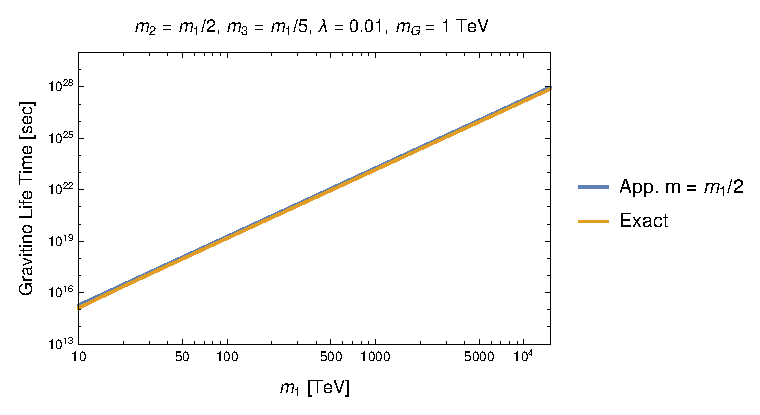
\includegraphics[scale=0.8]{GravitinoDecaym1m2m3Final}
\par\end{centering}

\caption{\label{fig:Gravitino-life-time}Gravitino life time in Trilinear RpV
for $\lambda_{ijk}=0.01,\,m_{G}=1\,\mbox{TeV}$. For simplicity we
use $m_{1},\,m_{2},\,m_{3}$ and $m$ instead of $m_{\tilde{\nu}_{iL}},\,m_{\tilde{e}_{jL}},\,m_{\tilde{e}_{kR}}$
and $\tilde{m}$.}
\end{figure}


Therefore, we can confidently derive the following expression for
the gravitino lifetime,

\begin{equation}
\tau_{G}\approx7\times10^{28}\,\mbox{sec}\,\left(\frac{1}{\lambda_{ijk}\lambda_{ijk}}\right)\left(\frac{\tilde{m}}{10^{8}\mbox{\,GeV}}\right)^{4}\left(\frac{1\,\mbox{TeV}}{m_{G}}\right)^{7}\label{eq:GravLifeTime}
\end{equation}


\noindent where we have normalized with respect to $10^{28}\mbox{ sec}$
since this is the order of magnitude required by experiments such
as AMS-02 and Fermi-LAT in order to fit the electron positron data
in the first case or to avoid gamma ray constraints in the second.


%\subsection{Neutrino Masses}

In trilinear RpV the neutrino mass matrix receives contributions from
1-loop diagrams that contain both a charged lepton and the corresponding
slepton. Indeed, we have derived the following (preliminary) expression

\begin{eqnarray*}
M_{ij}^{\nu\,(1)} & \approx & \frac{1}{16\pi^{2}}\sum_{gr}s_{\tilde{l}}c_{\tilde{l}}(\lambda_{igr}\lambda_{jrg}+\lambda_{jgr}\lambda_{irg})m_{g}\ln\frac{m_{\tilde{l}_{r2}}^{2}}{m_{\tilde{l}_{r1}}^{2}}
\end{eqnarray*}


\noindent where $i$ and $j$ are neutrino generation indices that
run from 1 to 3. $g$ is a charged lepton index that also run from
1 to 3, as well as $r$ which is a slepton index. Thus, it can be
seen that for order one $s_{\tilde{l}}$, $c_{\tilde{l}}$ and $\ln(m_{l_{r2}}^{2}/m_{l_{r1}}^{2})$
we can get neutrino masses around the eV scale for $\lambda_{ijk}\approx0.01$
even for $m_{g}\approx m_{e}$. 

Indeed, by following the expressions given in hep-ph/0410242 for the
contribution of $\lambda'$ trilinear terms, we can get by analogy
that the dominant term in the leptonic sector is 

\begin{eqnarray*}
M_{ij}^{\nu\,(1)} & \approx & \frac{1}{8\pi^{2}}\lambda_{i23}\lambda_{j32}\frac{m_{\mu}m_{\tau}A_{\tau}}{\tilde{m}^{2}}\\
 & \approx & 2\times10^{-2}\mbox{eV}\,\lambda_{i23}\lambda_{j32}\,\left(\frac{10^{8}\mbox{\,GeV}}{\tilde{m}}\right)\\
 & \approx & 2\times10^{-2}\mbox{eV}\,(\lambda_{i23}\lambda_{j32})^{5/4}\left(\frac{\tau_{G}}{7\times10^{\text{28}}\,\mbox{sec}}\right)^{1/4}\left(\frac{m_{G}}{1\,\mbox{TeV}}\right)^{7/4}
\end{eqnarray*}


\noindent where $A_{\tau}$ is a free parameter that can be considered
of order $\tilde{m}$, as it is done in hep-ph/0410242. Thus, if we
consider this formula together with Eq. \ref{eq:GravLifeTime} we
see that we can have contributions to the neutrino mass matrix of
order $10^{-2}\mbox{eV}$ for trilinear couplings and a scalar mass
which are compatible with $\tau_{G}\approx10^{28}\mbox{ sec}$.


\section*{Acknowledgments}

{\small 
The authors are thankful to Andrea Albert, Borut Bajc, Marco Cirelli, Michael Grefe, Luis Labarga, Carlos Munoz, Paolo Panci, Frank Steffen, and Gabriela Zaharijas for useful comments, and Marco Ajello for providing the EGB model contributions of figure~\ref{fig:EGBb}.
 This work was supported by Conicyt Anillo grant ACT1102. GAGV thanks for the support of the Spanish MINECO's Consolider-Ingenio 2010 Programme under grant MultiDark CSD2009-00064 also the partial support by MINECO under grant FPA2012-34694. BP also thanks for the support of the State of S\~{a}o Paulo Research Foundation (FAPESP). The work of NV was supported by CONICYT FONDECYT/POSTDOCTORADO/3140559.
}
%%%%%%%%%%%%%%%%%%%%%%%%%%%%%%%%%%%%%%%%%%%%%%%%%%%%%%%%%%%%%%%%%%

\bibliographystyle{JHEP}
\bibliography{Gravitino_Trilinear_References}

\end{document}


